\documentclass[11pt]{article}

\usepackage{amsmath,amssymb}	% for mathematical notation
\usepackage{float} 				% put things exactly where I tell you!
\usepackage{multicol} 			% for column layout
\usepackage[utf8]{inputenc} 	% can we has UTF-8, plox
\usepackage{listings}           % for embedded code
\usepackage{graphicx}           % for pretty pictures

\title%
{%
	{\large Miniprojekt}\\
	Biludlejning
}

\author%
{%
	Andreas Dall Løfgren\\
	\and
	Stine Knarkegaard Andersen\\
	\and
	Chris Dan Justesen\\
}

\begin{document}
\maketitle
\pagebreak
\tableofcontents

\section*{Systemudvikling}
\begin{figure}
  \centering
  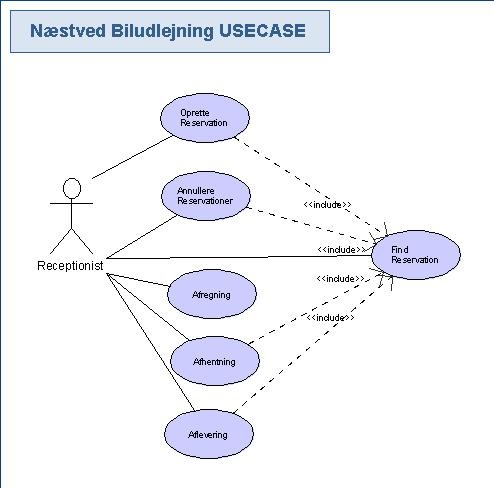
\includegraphics[width=10cm]{Naestved_Biludlejning_USECASE.jpeg}
  \caption{Use-case diagram}
  \label{fig:Use-case diagram}
\end{figure}

\begin{tabular}{ l | p{10cm} }
Oprette reservation & Oprettelse af reservationer ved indtastning af kundeoplysninger og biloplysninger. Laver en lejekontrakt. \\ \hline
Annullere reservationer & Annullering af reservation, hvis en reservation skal slettes. \\ \hline
Afregning & Den samlede afregning for lejen. \\ \hline
Afhentning & Kunden afhenter bilen. Bilens korte kilometer skal noteres.\\ \hline
Aflevering & Aflevering af bilen. Mængden af benzin og det kørte antal kilometer skal noteres. \\ \hline
\end{tabular}\\

Af disse funktioner da er oprettelse af reservationer den vigtigste, da den er påkrævet for at de andre fungerer.\\

Successcenarie for Oprettelse af reservation:
\begin{enumerate}
\item Kunden siger hvilken periode og prisgruppe han er interesseret i.
\item En liste over ledige biler kommer frem.
\item Man kommer til kundeoplysninger, der bliver skrevet ind.
\item Den færdige lejekontrakt bliver lavet og kan eventuelt printes.\\
\end{enumerate}

 Specialscenarie for Oprettelse af reservation:
\begin{enumerate}
\item Kunden siger hvilken periode og prisgruppe han er interesseret i.
\item Hvis der ikke er nogle ledige biler i den prisgruppe, da vil der ikke komme nogle biler frem.
\end{enumerate}

Løsningen er at tilbyde en bil fra en anden prisgruppe.

\end{document}